% Closed-loop form v2: the subtraction shown as a rewiring, not asserted as an equation.
% v1 drew the machine loop and the residual form and put an identity between them, so the
% equality was a claim in a label. v2 draws the derivation: (b) the loop we want, (c) the one
% step that uses linearity, (d) the result. The plant/model position is ONE opaque block F in
% all four panels, so the reader can see F is never split, inverted or linearised while the
% wires move around it. v1 is kept: it is the compact version for the write-up body.
% Dropped from v1 deliberately: the xc = 0 annotation (a different claim, it diluted this one)
% and the grey region (redundant once the Cfb blocks are visibly the only things manipulated).
% Style: figure-style.md, notation from jan-blockscheme-v4 and the closed-loop table in README.
% Compile: pdflatex closed-loop-form-v2.tex
\documentclass[border=12pt]{standalone}
\usepackage{tikz}
\usetikzlibrary{arrows.meta, calc}
\usepackage{amsmath}

\begin{document}
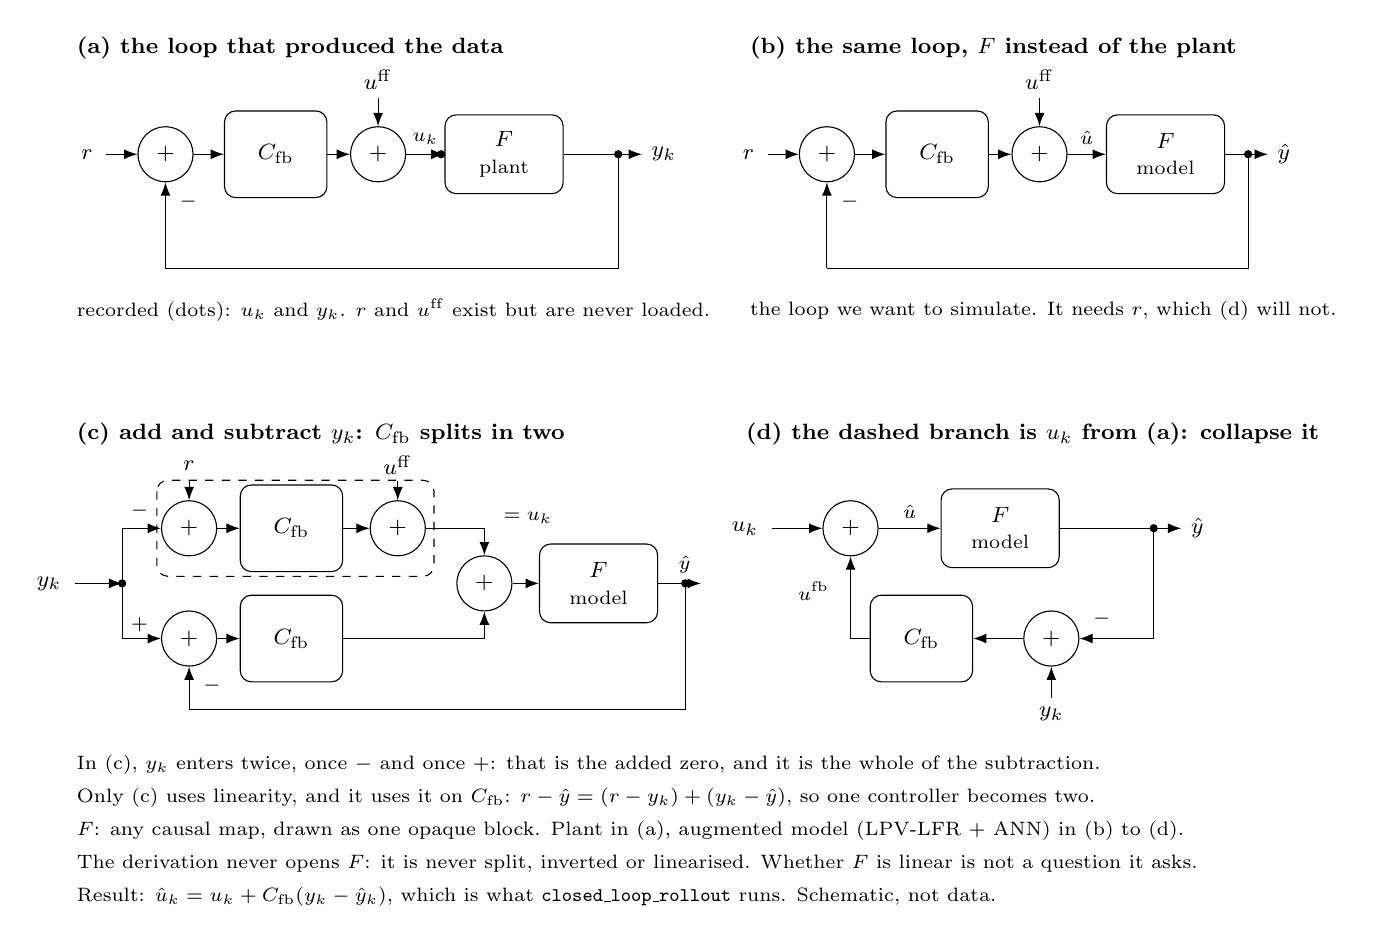
\begin{tikzpicture}[>=Latex, font=\footnotesize,
  block/.style={draw, rounded corners, minimum width=26mm, minimum height=12mm, align=center},
  rblock/.style={draw, rounded corners, minimum width=13mm, minimum height=11mm, align=center},
  small/.style={draw, rounded corners, minimum width=15mm, minimum height=10mm, align=center},
  sum/.style={draw, circle, minimum size=7mm, inner sep=0pt},
  jn/.style={circle, fill, minimum size=3pt, inner sep=0pt}]

% =================================================================================
% (a) the machine loop.  F = plant.
% =================================================================================
\node[anchor=west, font=\footnotesize\bfseries] at (-0.90,1.35)
  {(a) the loop that produced the data};

\node[sum]    (ae) at (0.35,0) {$+$};
\node[rblock] (ac) at (1.75,0) {$C_{\mathrm{fb}}$};
\node[sum]    (af) at (3.05,0) {$+$};
\node[small]  (aF) at (4.65,0) {$F$\\{\scriptsize plant}};

\node[left] at (-0.45,0) {$r$};
\draw[->] (-0.40,0) -- (ae.west);
\node at (3.05,0.95) {$u^{\mathrm{ff}}$};
\draw[->] (3.05,0.72) -- (af.north);

\draw[->] (ae.east) -- (ac.west);
\draw[->] (ac.east) -- (af.west);
\draw[->] (af.east) -- (aF.west) node[pos=0.5,above]{\scriptsize $u_k$};
\draw[->] (aF.east) -- (6.40,0) node[right]{$y_k$};
\node[jn] at (3.85,0) {};
\node[jn] at (6.10,0) {};
\draw[-]  (6.10,0) -- (6.10,-1.45) -- (0.35,-1.45);
\draw[->] (0.35,-1.45) -- (ae.south);
\node[font=\scriptsize] at (0.64,-0.60) {$-$};

\node[anchor=west, font=\scriptsize] at (-0.90,-1.98)
  {recorded (dots): $u_k$ and $y_k$. $r$ and $u^{\mathrm{ff}}$ exist but are never loaded.};

% =================================================================================
% (b) the same loop, F in place of the plant.  IDENTICAL geometry to (a).
% =================================================================================
\begin{scope}[xshift=-0.30cm]
\node[anchor=west, font=\footnotesize\bfseries] at (7.95,1.35)
  {(b) the same loop, $F$ instead of the plant};

\node[sum]    (be) at (9.05,0) {$+$};
\node[rblock] (bc) at (10.45,0) {$C_{\mathrm{fb}}$};
\node[sum]    (bf) at (11.75,0) {$+$};
\node[small]  (bF) at (13.35,0) {$F$\\{\scriptsize model}};

\node[left] at (8.25,0) {$r$};
\draw[->] (8.30,0) -- (be.west);
\node at (11.75,0.95) {$u^{\mathrm{ff}}$};
\draw[->] (11.75,0.72) -- (bf.north);

\draw[->] (be.east) -- (bc.west);
\draw[->] (bc.east) -- (bf.west);
\draw[->] (bf.east) -- (bF.west) node[pos=0.5,above]{\scriptsize $\hat u$};
\draw[->] (bF.east) -- (14.65,0) node[right]{$\hat y$};
\node[jn] at (14.40,0) {};
\draw[-]  (14.40,0) -- (14.40,-1.45) -- (9.05,-1.45);
\draw[->] (9.05,-1.45) -- (be.south);
\node[font=\scriptsize] at (9.34,-0.60) {$-$};

\node[anchor=west, font=\scriptsize] at (7.95,-1.98)
  {the loop we want to simulate. It needs $r$, which (d) will not.};
\end{scope}

% =================================================================================
% (c) add and subtract y_k.  THE step. One Cfb becomes two.
% =================================================================================
\node[anchor=west, font=\footnotesize\bfseries] at (-0.90,-3.55)
  {(c) add and subtract $y_k$: $C_{\mathrm{fb}}$ splits in two};

% the branch that will collapse
\draw[dashed, rounded corners] (0.24,-4.14) rectangle (3.76,-5.36);

\node[sum]    (ce)  at (0.65,-4.75) {$+$};
\node[rblock] (cc1) at (1.95,-4.75) {$C_{\mathrm{fb}}$};
\node[sum]    (cu1) at (3.30,-4.75) {$+$};
\node[sum]    (ce2) at (0.65,-6.15) {$+$};
\node[rblock] (cc2) at (1.95,-6.15) {$C_{\mathrm{fb}}$};
\node[sum]    (cu2) at (4.40,-5.45) {$+$};
\node[small]  (cF)  at (5.85,-5.45) {$F$\\{\scriptsize model}};

% r and u_ff enter the dashed branch from outside
\node at (0.65,-3.95) {$r$};
\draw[->] (0.65,-4.15) -- (ce.north);
\node at (3.30,-3.95) {$u^{\mathrm{ff}}$};
\draw[->] (3.30,-4.15) -- (cu1.north);

% y_k feeds BOTH error junctions, once minus and once plus: the added zero
\node[left] at (-0.85,-5.45) {$y_k$};
\draw[->] (-0.80,-5.45) -- (-0.20,-5.45);
\draw[-]  (-0.20,-4.75) -- (-0.20,-6.15);
\node[jn] at (-0.20,-5.45) {};
\draw[->] (-0.20,-4.75) -- (ce.west);
\draw[->] (-0.20,-6.15) -- (ce2.west);
\node[font=\scriptsize] at (0.02,-4.53) {$-$};
\node[font=\scriptsize] at (0.02,-5.97) {$+$};

\draw[->] (cc1.east) -- (cu1.west);
\draw[->] (ce.east)  -- (cc1.west);
\draw[->] (ce2.east) -- (cc2.west);
\draw[-]  (cu1.east) -- (4.40,-4.75);
\draw[->] (4.40,-4.75) -- (cu2.north);
\node[anchor=west, font=\scriptsize] at (4.52,-4.62) {$=u_k$};
\draw[-]  (cc2.east) -- (4.40,-6.15);
\draw[->] (4.40,-6.15) -- (cu2.south);
\draw[->] (cu2.east) -- (cF.west);
\draw[->] (cF.east) -- (7.15,-5.45) node[pos=0.62,above]{\scriptsize $\hat y$};
\node[jn] at (6.95,-5.45) {};
\draw[-]  (6.95,-5.45) -- (6.95,-7.05) -- (0.65,-7.05);
\draw[->] (0.65,-7.05) -- (ce2.south);
\node[font=\scriptsize] at (0.94,-6.75) {$-$};

% =================================================================================
% (d) collapse the dashed branch back into the recorded u_k.
% =================================================================================
\begin{scope}[xshift=-0.30cm]
\node[anchor=west, font=\footnotesize\bfseries] at (7.90,-3.55)
  {(d) the dashed branch is $u_k$ from (a): collapse it};

\node[sum]    (du) at (9.35,-4.75) {$+$};
\node[small]  (dF) at (11.25,-4.75) {$F$\\{\scriptsize model}};
\node[sum]    (de) at (11.90,-6.15) {$+$};
\node[rblock] (dc) at (10.25,-6.15) {$C_{\mathrm{fb}}$};

\node[left] at (8.30,-4.75) {$u_k$};
\draw[->] (8.35,-4.75) -- (du.west);
\draw[->] (du.east) -- (dF.west) node[pos=0.5,above]{\scriptsize $\hat u$};
\draw[->] (dF.east) -- (13.55,-4.75) node[right]{$\hat y$};
\node[jn] at (13.20,-4.75) {};
\draw[-]  (13.20,-4.75) -- (13.20,-6.15);
\draw[->] (13.20,-6.15) -- (de.east);
\node[font=\scriptsize] at (12.54,-5.90) {$-$};

\node[below] at (11.90,-6.90) {$y_k$};
\draw[->] (11.90,-6.90) -- (de.south);

\draw[->] (de.west) -- (dc.east);
\draw[-]  (dc.west) -- (9.35,-6.15);
\draw[->] (9.35,-6.15) -- (du.south);
\node[left, font=\scriptsize] at (9.20,-5.55) {$u^{\mathrm{fb}}$};
\end{scope}

% =================================================================================
% notes
% =================================================================================
\node[anchor=west, align=left, font=\scriptsize] at (-0.90,-7.75)
  {In (c), $y_k$ enters twice, once $-$ and once $+$: that is the added zero, and it is the
   whole of the subtraction.};
\node[anchor=west, align=left, font=\scriptsize] at (-0.90,-8.17)
  {Only (c) uses linearity, and it uses it on $C_{\mathrm{fb}}$:
   $r-\hat y=(r-y_k)+(y_k-\hat y)$, so one controller becomes two.};
\node[anchor=west, align=left, font=\scriptsize] at (-0.90,-8.59)
  {$F$: any causal map, drawn as one opaque block. Plant in (a), augmented model
   (LPV-LFR $+$ ANN) in (b) to (d).};
\node[anchor=west, align=left, font=\scriptsize] at (-0.90,-9.01)
  {The derivation never opens $F$: it is never split, inverted or linearised. Whether
   $F$ is linear is not a question it asks.};
\node[anchor=west, align=left, font=\scriptsize] at (-0.90,-9.43)
  {Result: $\hat u_k=u_k+C_{\mathrm{fb}}(y_k-\hat y_k)$, which is what
   \texttt{closed\_loop\_rollout} runs. Schematic, not data.};

\end{tikzpicture}
\end{document}
